% A LaTeX (non-official) template for ISAE projects reports
% Copyright (C) 2014 Damien Roque
% Version: 0.2
% Author: Damien Roque <damien.roque_AT_isae.fr>

% Updated version for Ensimag homework reports by Yoan Souty

\documentclass[a4paper,12pt, openany, twoside]{article}
\usepackage[utf8]{inputenc}
\usepackage[T1]{fontenc}
\usepackage[frenchb]{babel} % If you write in French
%\usepackage[english]{babel} % If you write in English
\usepackage{a4wide}
\usepackage{lipsum}
\usepackage{graphicx}
\usepackage{textcomp}
\graphicspath{{images/}} % emplacement des images
\usepackage{subfig}
 \usepackage{float}
\usepackage{tikz}
\usetikzlibrary{shapes,arrows}
\usepackage{pgfplots}
\pgfplotsset{compat=newest}
\pgfplotsset{plot coordinates/math parser=false}
\newlength\figureheight
\newlength\figurewidth
\pgfkeys{/pgf/number format/.cd,
set decimal separator={,\!},
1000 sep={\,},
}
\usepackage{ifthen}
\usepackage{ifpdf}
\ifpdf
\usepackage[pdftex]{hyperref}
\else
\usepackage{hyperref}
\fi
\usepackage{color}
\hypersetup{%
colorlinks=true,
linkcolor=black,
citecolor=black,
urlcolor=black}

\usepackage{titlesec}
\titleformat{\section}[hang]{\bf\huge}{\thesection}{2pc}{}

\renewcommand{\thesection}{\Roman{section}}


\renewcommand{\baselinestretch}{1.05}
\usepackage{fancyhdr}
% \pagestyle{fancy}
% \renewcommand{\sectionmark}[1]{\markboth{\thesection .\ #1}{}}
% \renewcommand{\subsectionmark}[1]{\markright{\thesubsection .\ #1}}
% \fancyhead{}
% \fancyhead[RE]{\nouppercase{\leftmark}}
% \fancyhead[LO]{\nouppercase{\rightmark}}
% \renewcommand{\headrulewidth}{0pt}

\let\headruleORIG\headrule
\renewcommand{\headrule}{\color{black} \headruleORIG}
\renewcommand{\headrulewidth}{1.0pt}
\usepackage{colortbl}
\arrayrulecolor{black}

% \fancypagestyle{plain}{
%   \fancyhead{}
%   \fancyfoot[C]{\thepage}
%   \renewcommand{\headrulewidth}{0pt}
% }

\makeatletter
\def\@textbottom{\vskip \z@ \@plus 1pt}
\let\@texttop\relax
\makeatother

\makeatletter
\def\cleardoublepage{\clearpage\if@twoside \ifodd\c@page\else%
  \hbox{}%
  \thispagestyle{empty}%
  \newpage%
  \if@twocolumn\hbox{}\newpage\fi\fi\fi}
\makeatother

\usepackage{amsthm}
\usepackage{amssymb,amsmath,bbm}
\usepackage{array}
\usepackage{bm}
\usepackage{multirow}
\usepackage[footnote]{acronym}

\newcommand*{\SET}[1]  {\ensuremath{\mathbf{#1}}}
\newcommand*{\VEC}[1]  {\ensuremath{\boldsymbol{#1}}}
\newcommand*{\FAM}[1]  {\ensuremath{\boldsymbol{#1}}}
\newcommand*{\MAT}[1]  {\ensuremath{\boldsymbol{#1}}}
\newcommand*{\OP}[1]  {\ensuremath{\mathrm{#1}}}
\newcommand*{\NORM}[1]  {\ensuremath{\left\|#1\right\|}}
\newcommand*{\DPR}[2]  {\ensuremath{\left \langle #1,#2 \right \rangle}}
\newcommand*{\calbf}[1]  {\ensuremath{\boldsymbol{\mathcal{#1}}}}
\newcommand*{\shift}[1]  {\ensuremath{\boldsymbol{#1}}}

\newcommand{\eqdef}{\stackrel{\mathrm{def}}{=}}
\newcommand{\argmax}{\operatornamewithlimits{argmax}}
\newcommand{\argmin}{\operatornamewithlimits{argmin}}
\newcommand{\ud}{\, \mathrm{d}}
\newcommand{\vect}{\text{Vect}}
\newcommand{\sinc}{\ensuremath{\mathrm{sinc}}}
\newcommand{\esp}{\ensuremath{\mathbb{E}}}
\newcommand{\hilbert}{\ensuremath{\mathcal{H}}}
\newcommand{\fourier}{\ensuremath{\mathcal{F}}}
\newcommand{\sgn}{\text{sgn}}
\newcommand{\intTT}{\int_{-T}^{T}}
\newcommand{\intT}{\int_{-\frac{T}{2}}^{\frac{T}{2}}}
\newcommand{\intinf}{\int_{-\infty}^{+\infty}}
\newcommand{\Sh}{\ensuremath{\boldsymbol{S}}}
\newcommand{\C}{\SET{C}}
\newcommand{\R}{\SET{R}}
\newcommand{\Z}{\SET{Z}}
\newcommand{\N}{\SET{N}}
\newcommand{\K}{\SET{K}}
\newcommand{\reel}{\mathcal{R}}
\newcommand{\imag}{\mathcal{I}}
\newcommand{\cmnr}{c_{m,n}^\reel}
\newcommand{\cmni}{c_{m,n}^\imag}
\newcommand{\cnr}{c_{n}^\reel}
\newcommand{\cni}{c_{n}^\imag}
\newcommand{\tproto}{g}
\newcommand{\rproto}{\check{g}}
\newcommand{\LR}{\mathcal{L}_2(\SET{R})}
\newcommand{\LZ}{\ell_2(\SET{Z})}
\newcommand{\LZI}[1]{\ell_2(\SET{#1})}
\newcommand{\LZZ}{\ell_2(\SET{Z}^2)}
\newcommand{\diag}{\operatorname{diag}}
\newcommand{\noise}{z}
\newcommand{\Noise}{Z}
\newcommand{\filtnoise}{\zeta}
\newcommand{\tp}{g}
\newcommand{\rp}{\check{g}}
\newcommand{\TP}{G}
\newcommand{\RP}{\check{G}}
\newcommand{\dmin}{d_{\mathrm{min}}}
\newcommand{\Dmin}{D_{\mathrm{min}}}
\newcommand{\Image}{\ensuremath{\text{Im}}}
\newcommand{\Span}{\ensuremath{\text{Span}}}

\newtheoremstyle{break}
  {11pt}{11pt}%
  {\itshape}{}%
  {\bfseries}{}%
  {\newline}{}%
\theoremstyle{break}

%\theoremstyle{definition}
\newtheorem{definition}{Définition}[section]

%\theoremstyle{definition}
\newtheorem{theoreme}{Théorème}[section]

%\theoremstyle{remark}
\newtheorem{remarque}{Remarque}[]

%\theoremstyle{plain}
\newtheorem{propriete}{Propriété}[section]
\newtheorem{exemple}{Exemple}[section]

\newtheorem{question}{Question}[section]

\parskip=5pt
%\sloppy

\begin{document}

%%%%%%%%%%%%%%%%%%
%%% First page %%%
%%%%%%%%%%%%%%%%%%

\begin{titlepage}
\begin{center}

\includegraphics[width=0.6\textwidth]{ensimag_logo.png}\\[1cm]

{\large Ensimag MMIS 3A}\\[0.5cm]

{\large Visualisation Scientifique}\\[0.5cm]

% Title
\rule{\linewidth}{0.5mm} \\[0.4cm]
{ \huge \bfseries Images commentées de la visualisation de données météo\\[0.4cm] }
\rule{\linewidth}{0.5mm} \\[1.5cm]

% Author and supervisor
\noindent
\begin{minipage}{0.4\textwidth}
  \begin{flushleft} \large
    \emph{Auteurs :}\\
    M. Antonin \textsc{Klopp-Tosser}\\
    M. Yoan \textsc{Souty} \\
  \end{flushleft}
\end{minipage}%
\begin{minipage}{0.4\textwidth}
  \begin{flushright} \large
    \emph{Encadrant :} \\
    %M\up{me} Valérie \textsc{Perrier} \\

    M.~Georges-Pierre \textsc{Bonneau}
  \end{flushright}
\end{minipage}

\vfill

% Bottom of the page
{\large \today}

\end{center}
\end{titlepage}

%%%%%%%%%%%%%%%%%%%%%%%%%%%%%
%%% Non-significant pages %%%
%%%%%%%%%%%%%%%%%%%%%%%%%%%%%


%%%%%%%%%%%%%%%%%%%%%%%%%%%%%%%%%%%%%%%%%%%%
%%% Content of the report and references %%%
%%%%%%%%%%%%%%%%%%%%%%%%%%%%%%%%%%%%%%%%%%%%

\pagestyle{fancy}


% \tableofcontents
%
% \clearpage
%
% \listoffigures
%
% \clearpage




\begin{figure}[H]
  \centering
  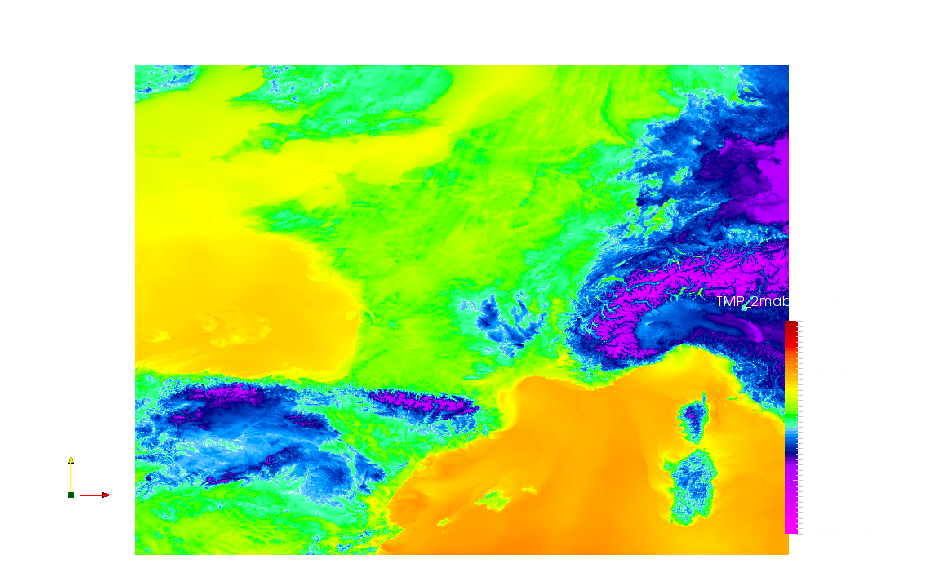
\includegraphics[width=0.7\textwidth]{1}
  \caption{Courbe iso-valeur, champs des températures et lignes de courant (SP1)}
\end{figure}
\vspace{-5mm}

Cette carte montre les températures sur la zone Europe, une courbe iso-valeur (en noire) et les lignes de
courant (en blanc) dans une direction particulière. Le choix des couleurs pour les températures est basé sur l'échelle de couleurs utilisée par MétéoFrance.

\begin{figure}[H]
  \centering
  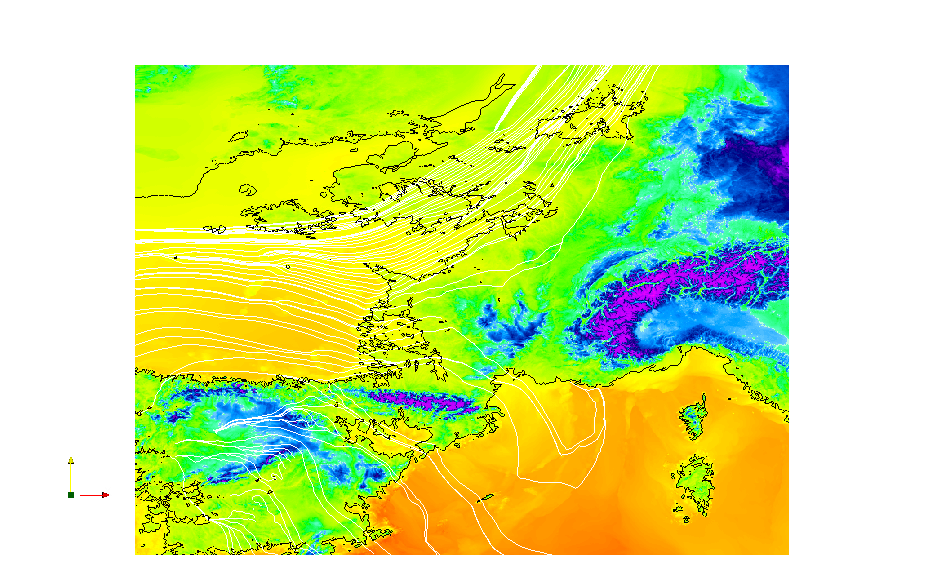
\includegraphics[width=0.7\textwidth]{2}
  \caption{Plusieurs courbes iso-valeurs (SP1)}
\end{figure}
\vspace{-5mm}

On affiche pour cette animation plusieurs courbes iso-valeurs, de façon à visualiser quelques zones de températures de 265\textdegree K ($\approx -8.15$\textdegree C) à 290 \textdegree K  ($\approx 16.85$\textdegree C) par pas de 5\textdegree K.


\begin{figure}[H]
  \centering
  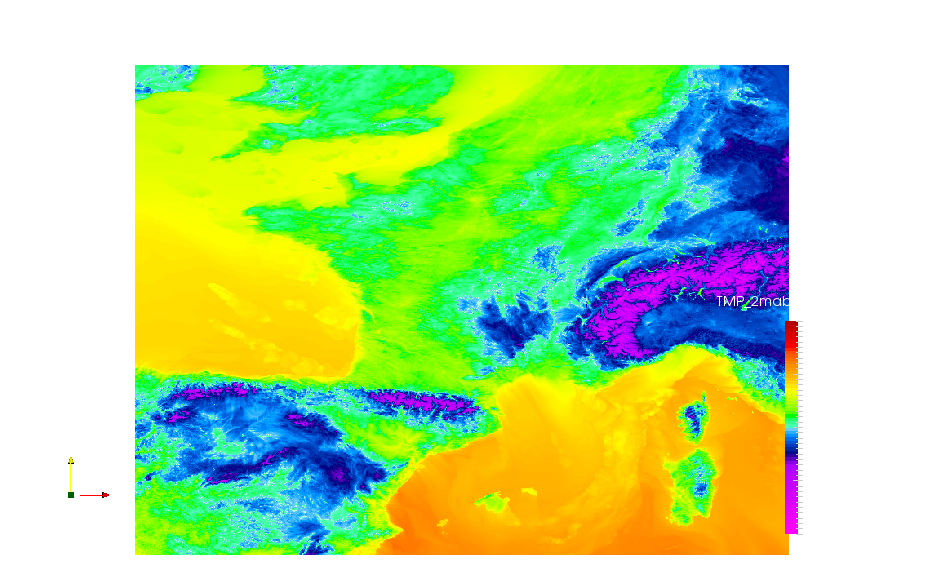
\includegraphics[width=0.7\textwidth]{3}
  \caption{Plusieurs champs de températures (SP1)}
\end{figure}
\vspace{-5mm}

Cette troisième animation permet de visualiser l'évolution des températures sur 6 heures. Les températures (à la date du 26 novembre 2018) vont de 271.358\textdegree K ($\approx -2.15$\textdegree C) en violet à 294\textdegree K ($\approx 20.85$\textdegree C) en orange-rouge. Sur l'animation lancée, on observe que les températures les plus chaudes sont localisées principalement en Europe méditerranénne, comme sur les carte des iso-valeurs.








\end{document}
